%%%% Introduction to LIGO

\section{Design of LIGO}\label{sec:ligo_construction}
\begin{figure}
 \begin{center}
  \scalebox{1}{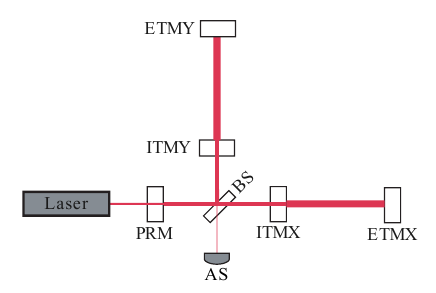
\includegraphics[width=0.6\columnwidth]{figures/ligo/ligo-schematic.png}} 
 \end{center}
\label{fig:ligo}
\caption{Schematic of interferometric detectors, like LIGO and Virgo.}
\end{figure}



\section{Dominant Noise Sources}\label{sec:ligo_noise}

We define the strain signal, $s$, to be the relative change in the length 
of the two arms of the interferometer
% 
\begin{equation}
 s(t) = \dfrac{\Delta L_x - \Delta L_y}{L}.
\end{equation}
% 
The signal $s(t)$ can be written as the sum of two components, (i) the actual
differential arm length change induced by the incident gravitational wave 
$h(t)$ (if present), and (ii) the sum of various noises, $n(t)$, that affect 
the measurement of the difference in the arm lengths $\Delta L$. 
%
As the goal of LIGO is to measure remarkably small length changes, several
sources of noise that propagate to the measurement of $s(t)$ become 
consequential. A few intrinsic to the instrument include the brownian motion
noise in mechanical systems, lossy optics, cross-talk in electromagnetic
systems, noise in control electronics, etc. Additionally, there are noise 
sources in the environment of the detectors, such as wind and ground motion,
fluctuations in the Newtonian gravity due to changes in atmosphere or ground
density, electric coupling from nearby power lines etc. 
%
It is therefore a challenging task to categorize these sources and reduce the
noise to the best extent possible.


Gravitational wave searches in LIGO data are affected by the {\it power
spectral density} of all the noise sources combined. The fundamental noise 
sources that limit the sensitivity of the interferometer in different frequency
ranges are:
% 
\begin{enumerate}
 \item Seismic noise:
 The motion of the ground, whether it be due to earthquakes or due to human 
 activity, couples mechanically to the suspended test masses. This coupling
 leads to fluctuation in the vertical and horizontal position of the suspended
 test masses at the end of each arm. The suspension of mirrors as pendula acts 
 as a low pass filter for seismic motion. There are active systems in place as
 well that sense ground motion and feed the information back to cancel its
 effect. Seismic noise affects the sensitivity of the detectors at frequecies
 $< 40$~Hz.
 \item (Suspension) thermal noise:
 Each degree of freedom has an expected energy that depends on the temperature,
 leading to thermal noise in the observations related to that dgree of freedom.
 The leading source of thermal noise is the molecular Brownian motion in the
 mirror suspension wires, and in the surface of the mirror. Thermal noise is 
 a low frequency noise that falls off inversely with frequency. It dominates
 the detector sensitivity in the range $\sim 40-150$~Hz.
 \item Photon shot noise:
 During operation, the interferometer is locked 
 with the optical fields from the two arms interfering destructively at the
 beam splitter, or in other words at a {\it dark fringe}. The number of photons
 that arrive at the readout will be directly proportional to the gravitational
 wave signal causing the arms to elongate or contract. The arrival times of the
 photons follows Poissonian statistics. Therefore the counting of the number of
 photons that arrive in a given interval of time, $\mathcal{N}$ will have an 
 inherent uncertainty that will be proportional to $\sqrt{\mathcal{N}}$.
 %
 In frequency domain, the shot noise has a flat (or {\it white}) spectrum. 
 However, the arms of the interferometer act as a filter and amplify the effect
 of the shot noise on our ability to measure the incident gravitational wave
 with increasing frequency. As a result, this noise source dominates over all
 others at $f\gtrsim 1$~kHz.
\end{enumerate}
% 
We refer the reader to the classic book by Saulson~\cite{Saulson:1995zi} for a
detailed treatment of these noise sources, which is out of scope of this 
dissertation. 

Apart from these continuous noise sources, there is another class of noise 
that plagues our ability to systematically extract signals embedded in detector
data called {\it glitches}. Glitches are transient by definition, and have a 
variety of frequency spectrum and sources. More importantly, if not correctly 
identified with their cause, they could be unpredictable. For instance, the 
falling of a 
heavy object could shake optics and lead to a sharp rise in the noise level
in the differential arm length output. There are mechanisms being developed to 
identify and classify glitches in Advanced LIGO and Virgo, within the Detector
characterization group. There are also algorithms in place that allow search 
methods to differentiate between signals and glitches based on their frequency
spectrum and evolution.


% This section is completely un-necessary
\section{Calibration of LIGO}\label{sec:ligo_calibration}
\begin{figure}
 \begin{center}
  \scalebox{1}{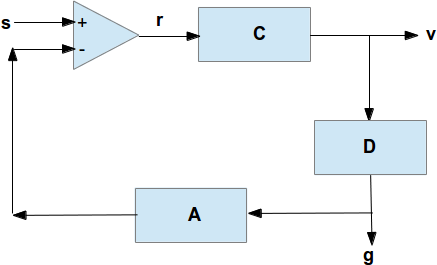
\includegraphics[width=0.6\columnwidth]{figures/ligo/ligo-control-loop.png}} 
 \end{center}
\label{fig:ligo_calibration}
\caption{Model for the control loop of the LIGO length sensing and control system.}
\end{figure}

The signal recorded at the output port $v(t)$ is proportional to the effect of 
the differential motion of the mirrors in the two arms of the interferometer.
This signal is itself used in a control loop to further stabilize the free-falling
masses by actuating on them. Therefore the effect of the gravitational waves alone, 
$s(t)$ has to be decoded from $v(t)$ by understanding this control loop.

Let us model this length sensing control loop as in
Fig.~\ref{fig:ligo_calibration}. All the blocks symbolize the transfer function
of a particular logical block, which is the ratio of its output to its input.
All quantities hereafter will be in frequency domain, while the transfer 
functions themselves could be slowly varying in time as well. 
Block $C$ denotes the 
length sensing function. It measures the response of the arm cavities to 
gravitational waves. Block $D$ converts the output of block $C$, i.e. the 
fluctuation in the differential arm length into a control signal that is sent
to block $A$. Block $A$ is the {\it actuation} function that reacts to the 
control signal and actuates upon the suspended masses in a way so as to 
stabilize them. 

We calculate the transfer function $G$ between the readout and the actual 
gravitational wave signal as
%
\begin{equation}
 \begin{split}
  v = C\, r ;\hspace{5mm} g &= D\, v = CD\, r ;\hspace{5mm} r = s - A\, g = s - CDA\, r, \\
  &\Rightarrow G \defeq \dfrac{s}{v} = \dfrac{1 + CDA}{C}.
 \end{split}
\end{equation}
% 
The process of calibrating interferometer data therefore involves measuring 
the aforementioned transfer functions to high accuracy and using them to obtain 
the final data channel containing the possible gravitational wave signal.



\section{Detector response to Gravitational wave polarizations}\label{sec:ligo_response}
\begin{figure}
 \begin{center}
  \scalebox{1}{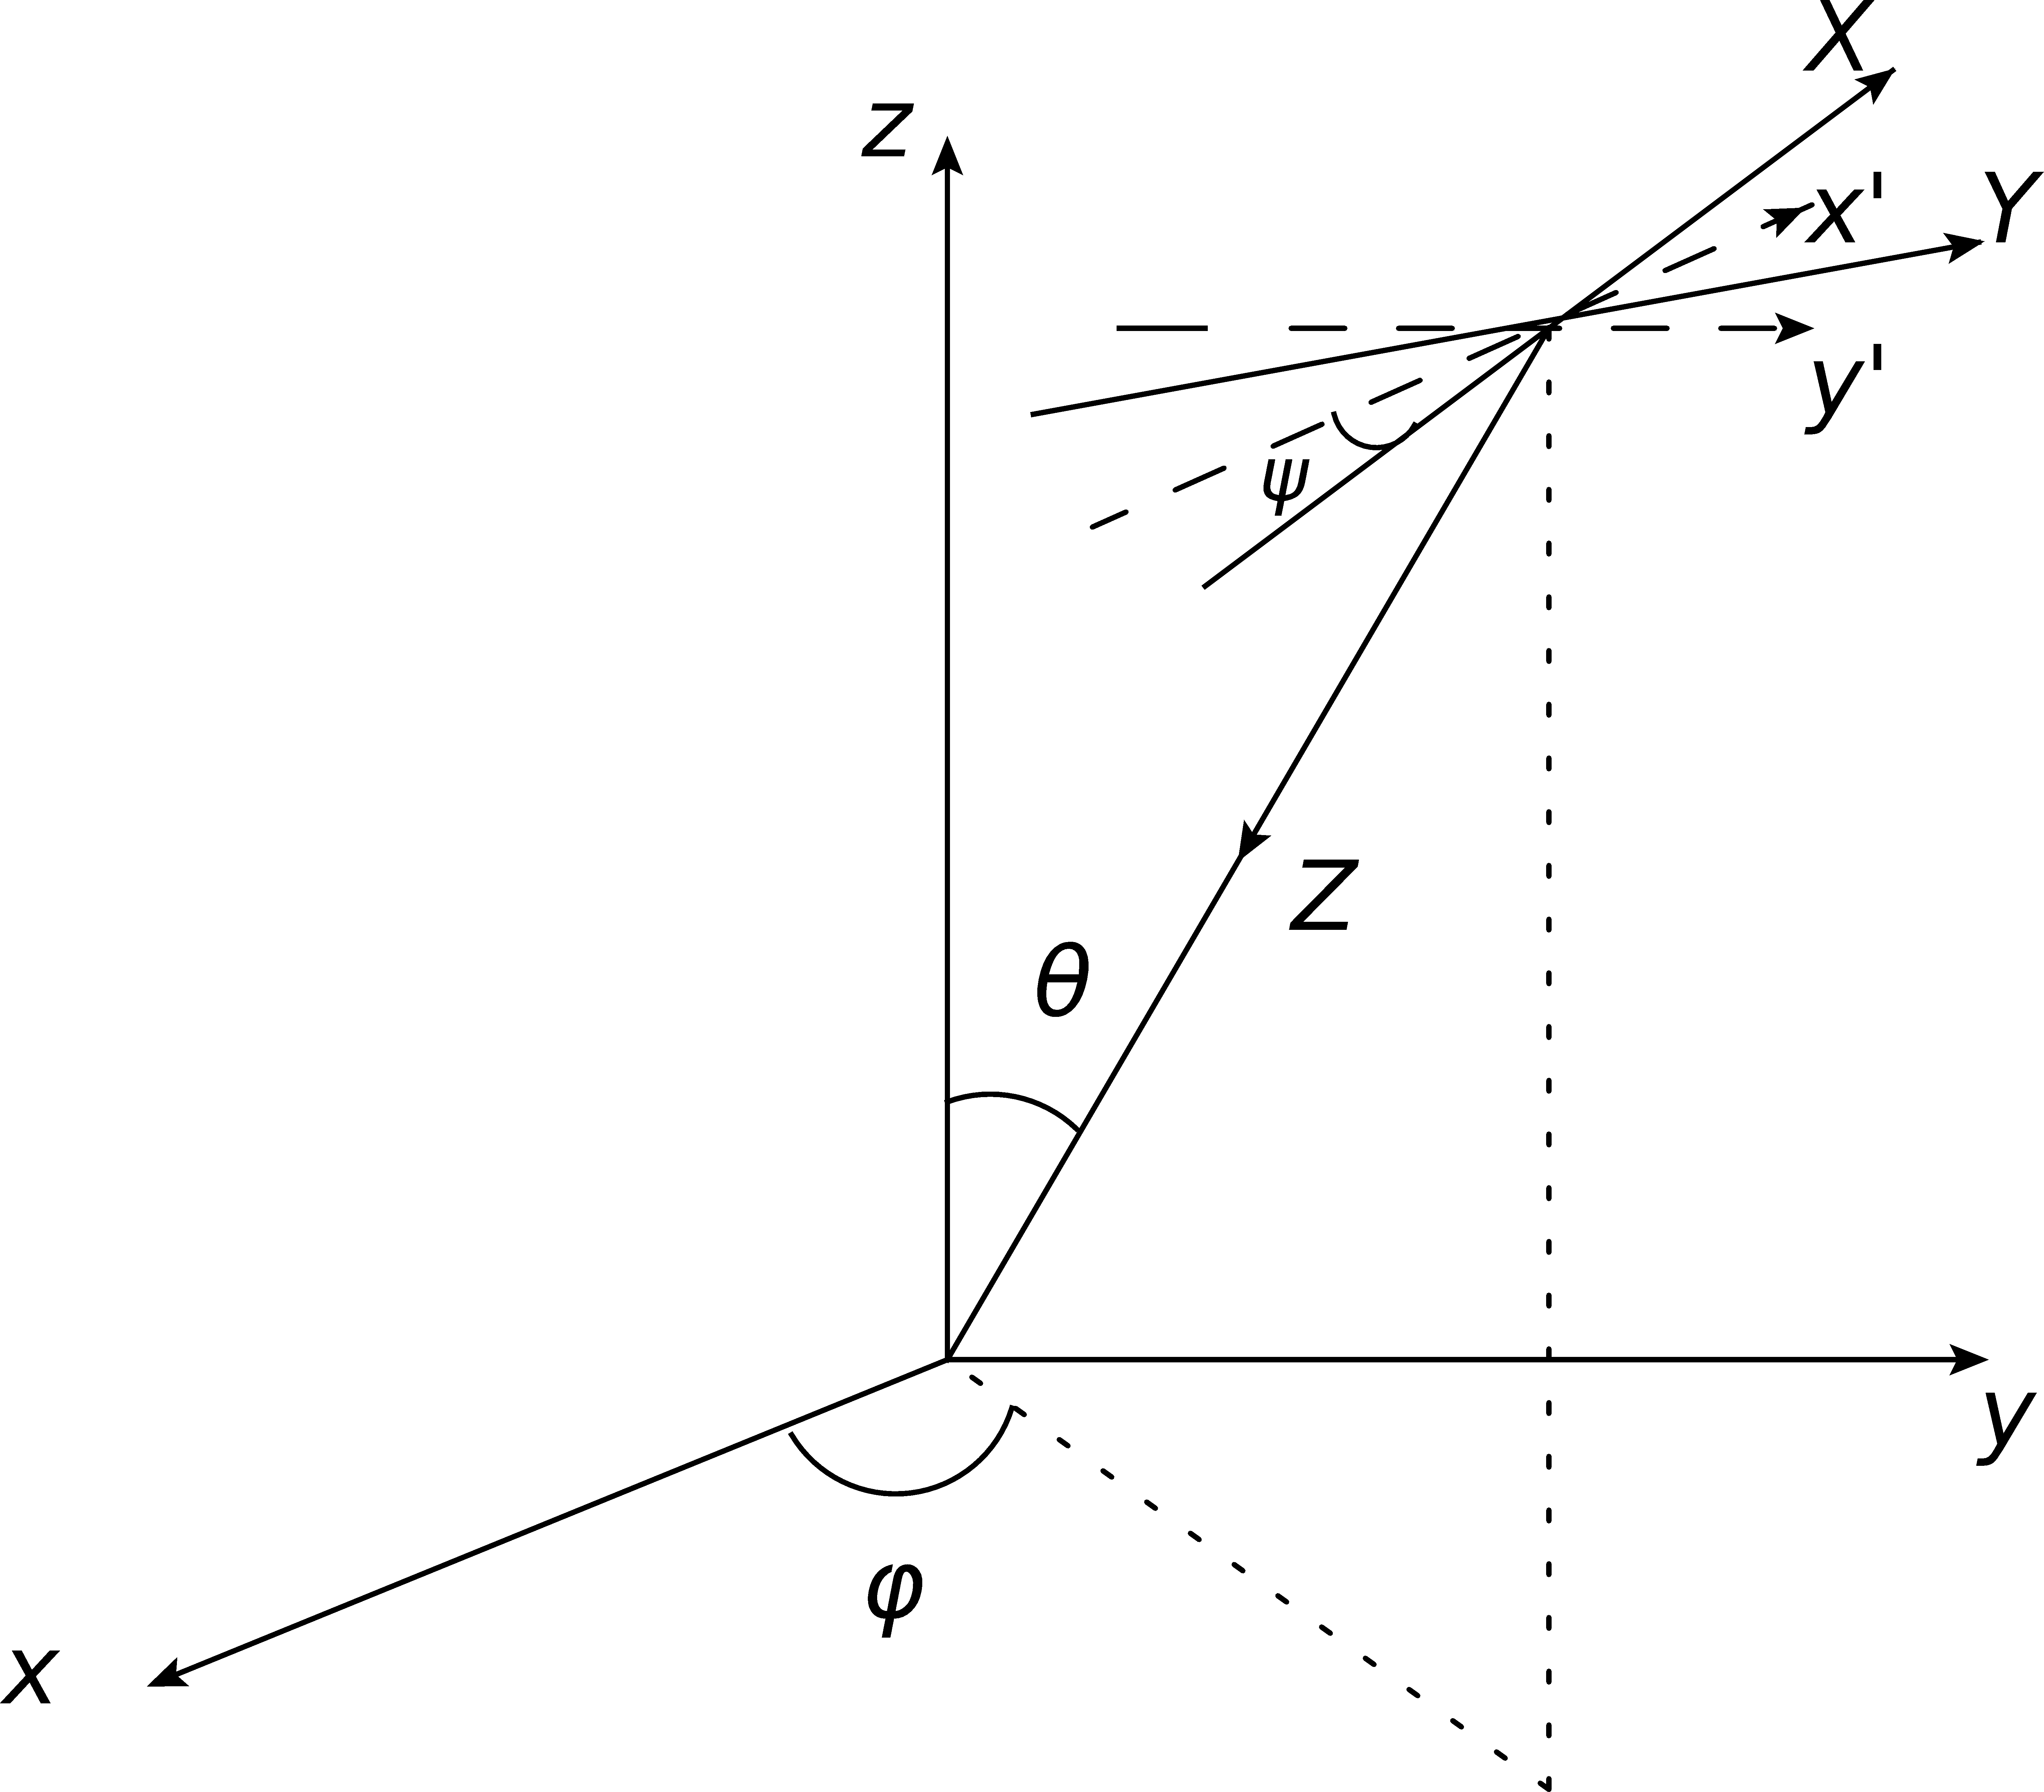
\includegraphics[width=0.6\columnwidth]{figures/ligo/radiation-detector-frame.png}} 
 \end{center}
\label{fig:radiation_detector_frames}
\caption{The Euler angles $\{\theta,\phi,\psi\}$ to go from teh gravitational 
wave propagation frame to the detector frame.}
\end{figure}

We start with defining the radiation frame which has its $x-y$ plane in the 
plane of the sky if one is looking towards the source. The line connecting the 
source and the detector defines its $z-$axis. Therefore we can determine the 
polar angles $(\theta,\phi)$ that point correspond to the $z-$axis of the 
radiation frame. Finally, we denote the angle between the $x-$axis of the 
radiation frame and the plane made by joining the $x-$arm of the detector and
the $z-$axis of the radiation frame. The detector frame is intuitively defined
by defining the $x$ and $y$ axes along the two arms with the $z-$axis coming
out of the plane of the detector on Earth.

It can be shown that the polarization amplitudes in the radiation frame depend 
on the {\it inclination} angle $\iota$ between the orbital (or total) angular 
momentum of the binary and the line of sight from the detector to the source
as~\cite{SathyaSchutzLRR}
% 
\begin{equation}\label{eq:h_inclination}
 h_+ = \frac{1}{2}(1 + \cos^2\iota)\,h_0\cos\Phi(t); \hspace{10mm} h_\times = \cos\iota\,h_0\sin\Phi(t).
\end{equation}
%
$h_0$ is an overall amplitude that varies slowly in time compared to the 
instantaneous gravitational wave phase $\Phi(t)$. 
In the radiation frame the tensorial metric perturbation can be written as 
(bold fonts indicate tensors or vectors with indices suppressed)
\begin{equation}
 {\bf h} = h_+{\bf e_+} + h_\times{\bf e_\times}
\end{equation}
% 
where the basis tensors are defined as
% 
\begin{equation}
 {\bf e_+}\defeq {\bf e^R_x}\otimes {\bf e^R_x} - {\bf e^R_y}\otimes {\bf e^R_y}; \hspace{10mm}
 {\bf e_\times}\defeq {\bf e^R_x}\otimes {\bf e^R_y} + {\bf e^R_y}\otimes {\bf e^R_x},
\end{equation}
% 
with ${\bf e^R_x}$ and ${\bf e^R_y}$ being unit vectors along the $x$ and $y$ 
axes of the radiation frame. Next we define the {\it detector tensor}, which 
can be thought of as the projection tensor for the detector, as
% 
\begin{equation}
 {\bf d} \defeq L({\bf e^D_x}\otimes {\bf e^D_x} - {\bf e^D_y}\otimes {\bf e^D_y}),
\end{equation}
% 
where ${\bf e^D_x}$ and ${\bf e^D_y}$ are unit vectors along the $x$ and $y$ 
axes of the detector frame, and they point along the direction of the arms from 
the central beam splitter. $L$ is the length of each arm of the interferometer. 
The change in length of the arms $\delta L(t)$ can therefore be obtained as the
scalar product between the ${\bf h}$ tensor and the detector tensor, i.e.
% 
\begin{equation}
 \delta L(t) = {\bf d}\cdot {\bf h} \defeq d_{ij}h^{ij}
\end{equation}
% 
This allows the strain produced in the arms to be written as
% 
\begin{equation}\label{eq:h_strain_antenna}
 h(t)\defeq\frac{\delta L}{L} = F_+(\theta, \phi, \psi) h_+ + F_\times(\theta, \phi, \psi) h_\times,
\end{equation}
where the functions $F_+$ and $F_\times$ can be found using the geometry in
Fig.~\ref{fig:radiation_detector_frames} as the scalar product of the basis tensors
${\bf e_+}$ and  ${\bf e_\times}$ with the detector tensor~\cite{SathyaSchutzLRR},
% 
\begin{equation}\label{eq:fpluscross}
 \begin{split}
  F_+ &= \frac{1}{2}(1 + \cos^2\theta)\cos(2\phi)\cos(2\psi) - \cos(\theta)\sin(2\phi)\sin(2\psi), \\
  F_\times &= \frac{1}{2}(1 + \cos^2(\theta))\cos(2\phi)\sin(2\psi) + \cos(\theta)\sin(2\phi)\cos(2\psi).
 \end{split}
\end{equation}
These two functions are called the {\it antenna patterns} of the detector, 
and they define the response of the detector to incoming gravitational 
radiation governed purely due to the relative geometry between the source and 
the detector itself. Finally, collecting Eq.~\eqref{eq:h_inclination} and
Eq.~\eqref{eq:h_strain_antenna} we can write the strain $h(t)$ seen by the 
detector as
% 
\begin{equation}
 h(t) = F_+ h_+ + F_\times h_\times = \mathcal{A} h_0 \cos(\Phi(t) - \Phi_0),
\end{equation}
% 
where $\Phi(t)$ has the same meaning as in Eq.~\eqref{eq:h_inclination}, and
% 
\begin{equation}
\begin{split}
 \mathcal{A} &\defeq \left(\left(\frac{1}{2}F_+(1+\cos^2\iota)\right)^2 + \left(F_\times\cos\iota\right)^2\right)^{1/2}, \\
 \Phi_0 &\defeq \tan^{-1}\left( \frac{2F_\times\cos\iota}{F_+(1+\cos^2\iota)}\right),
\end{split}
\end{equation}
% 
are combinations of the antenna patterns and the inclination angle folded 
into a constant amplitude and phase change. 

